\documentclass[12pt, letterpaper, titlepage, hidelinks]{article}

% Packages
\usepackage[letterpaper, margin=1in]{geometry}
\usepackage[utf8]{inputenc}
\usepackage{fancyhdr}
\usepackage{setspace}
\usepackage{amssymb}
\usepackage{amsmath}
\usepackage{multirow}
\usepackage{array}
\usepackage{graphicx}
\usepackage{tabularx}
\usepackage{booktabs}
\usepackage{hyperref}
\usepackage{scrextend}
\usepackage{verbatim}
\usepackage[english]{babel}
\usepackage{blindtext}
\usepackage{capt-of}
\usepackage{float}
\usepackage{caption}
\usepackage{apacite}
\usepackage{mathrsfs}
\usepackage{pdfpages}
\usepackage[autostyle, english = american]{csquotes}
\MakeOuterQuote{"}

\graphicspath{ {Images/} }


\newenvironment{nospaceflalign*}
{\setlength{\abovedisplayskip}{0px}\setlength{\belowdisplayskip}{0px}%
	\csname flalign*\endcsname}
{\csname endflalign*\endcsname\ignorespacesafterend}

% Title Page
\title{4DM4 Assignment 2 \\ Advanced Static Pipelining}
\author{Ashpan Raskar raskara 400185326\\
		Ahnaf Bhuiyan bhuiya3 400198359}
\date{\today}



\begin{document}

\maketitle
\tableofcontents
\newpage
\setlength{\parindent}{0pt}
\setcounter{secnumdepth}{0}
\section{Part (a): DAXPY Loop, No Unrolling, with No Scheduling}
	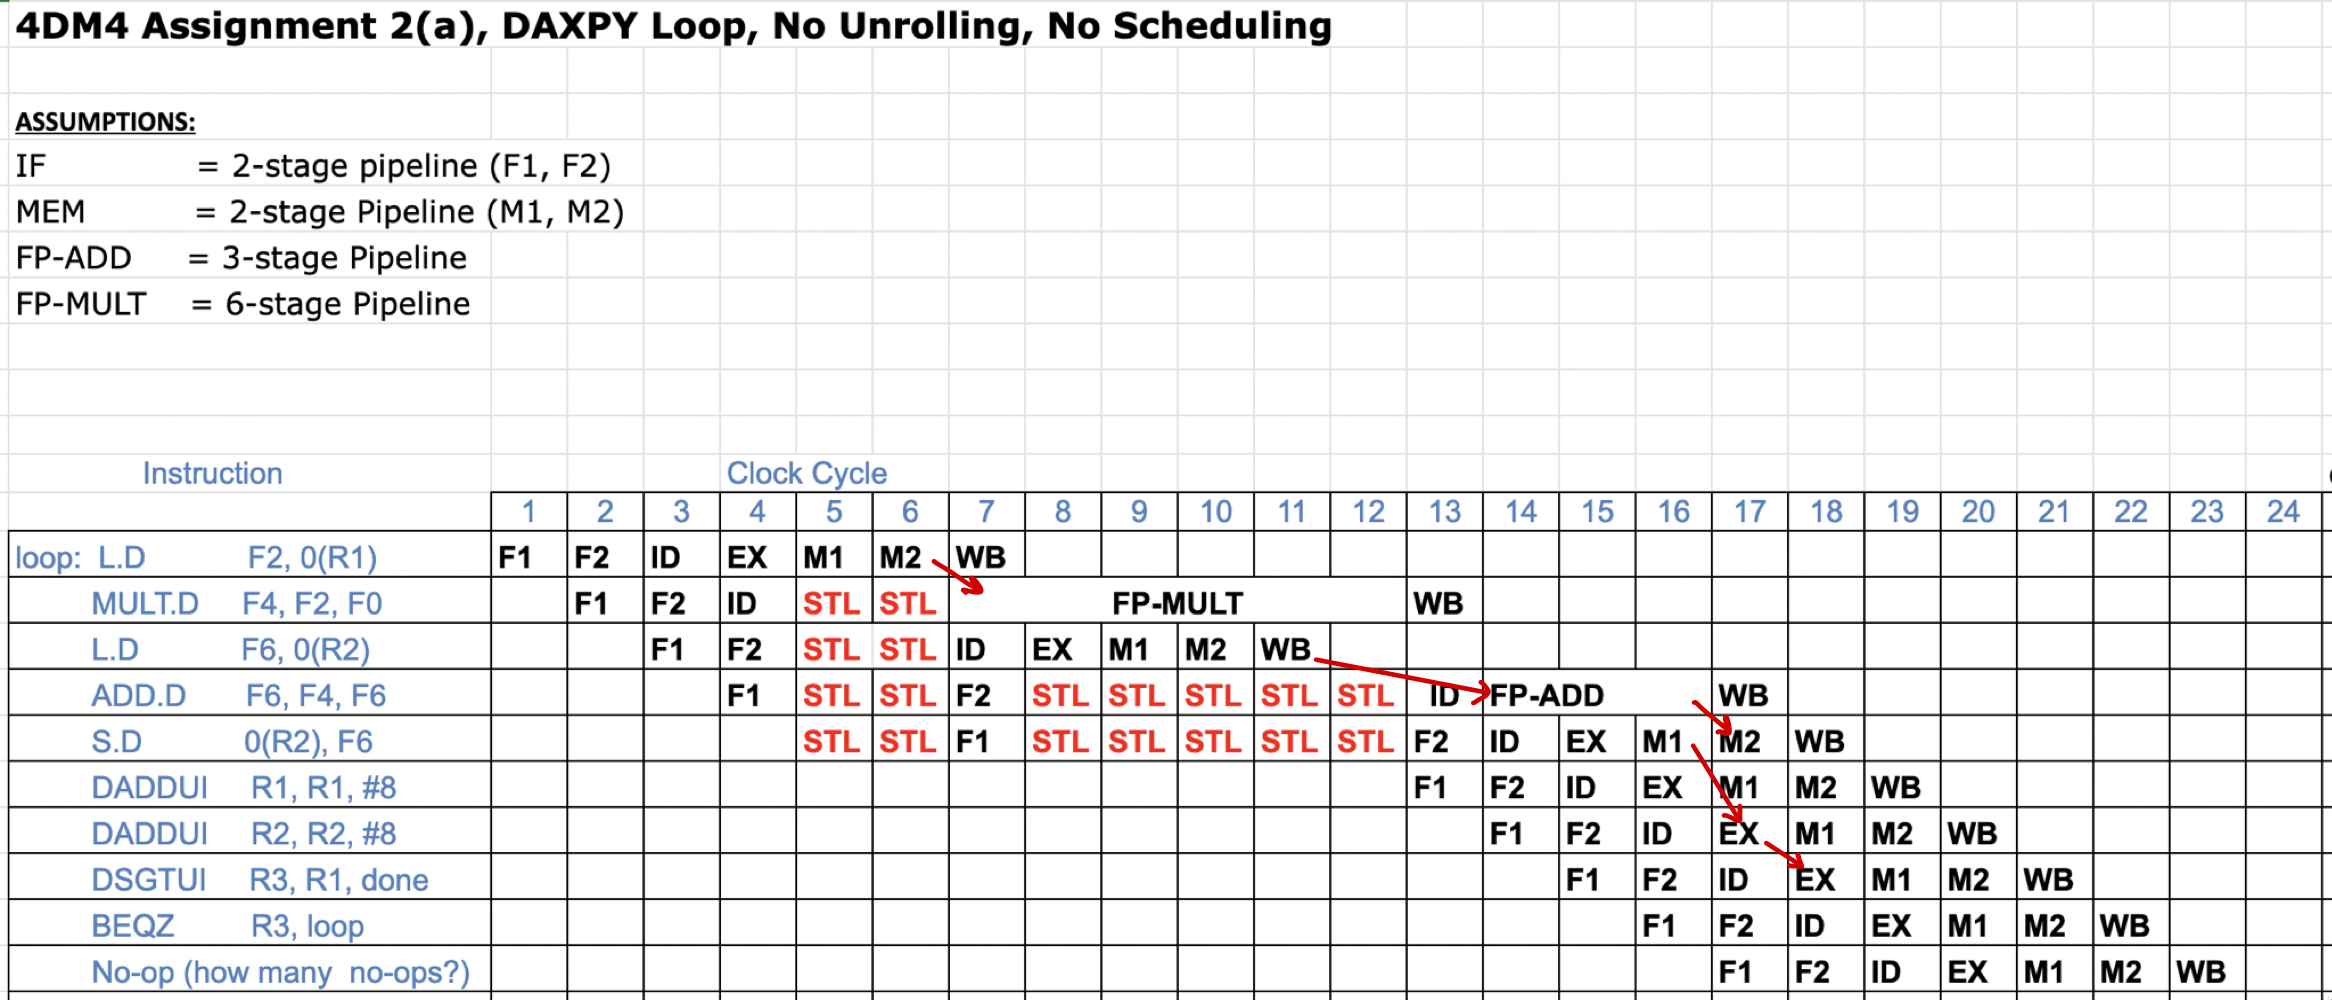
\includegraphics[width=\textwidth]{2a}
	Each iteration of this loop takes 23 clock cycles. The given clock speed is 3 GHz. The following equation can be used to calculate the MFLOP rating for this process.
	\begin{equation}
		\text{MFLOP Rating} = (3 \text{{Ghz}}) * \frac{1 \text{ FLOP}}{23 \text{ clock cycles}} = 130.4 \text{ MFLOP/s}
	\end{equation}
	% 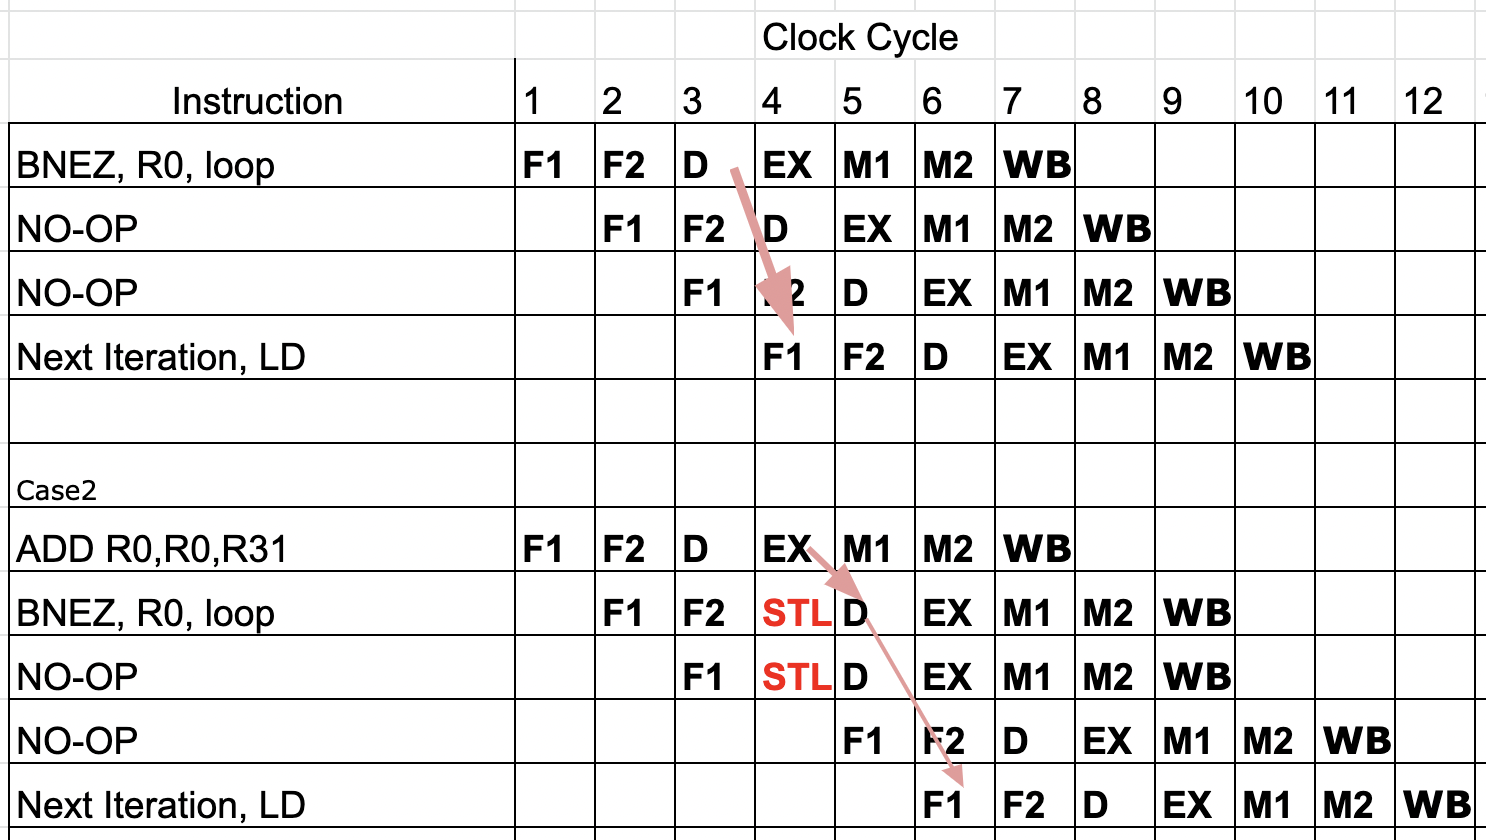
\includegraphics[width=\textwidth]{A2}
\section{Part (b): DAXPY Loop, No Unrolling, with Scheduling}
	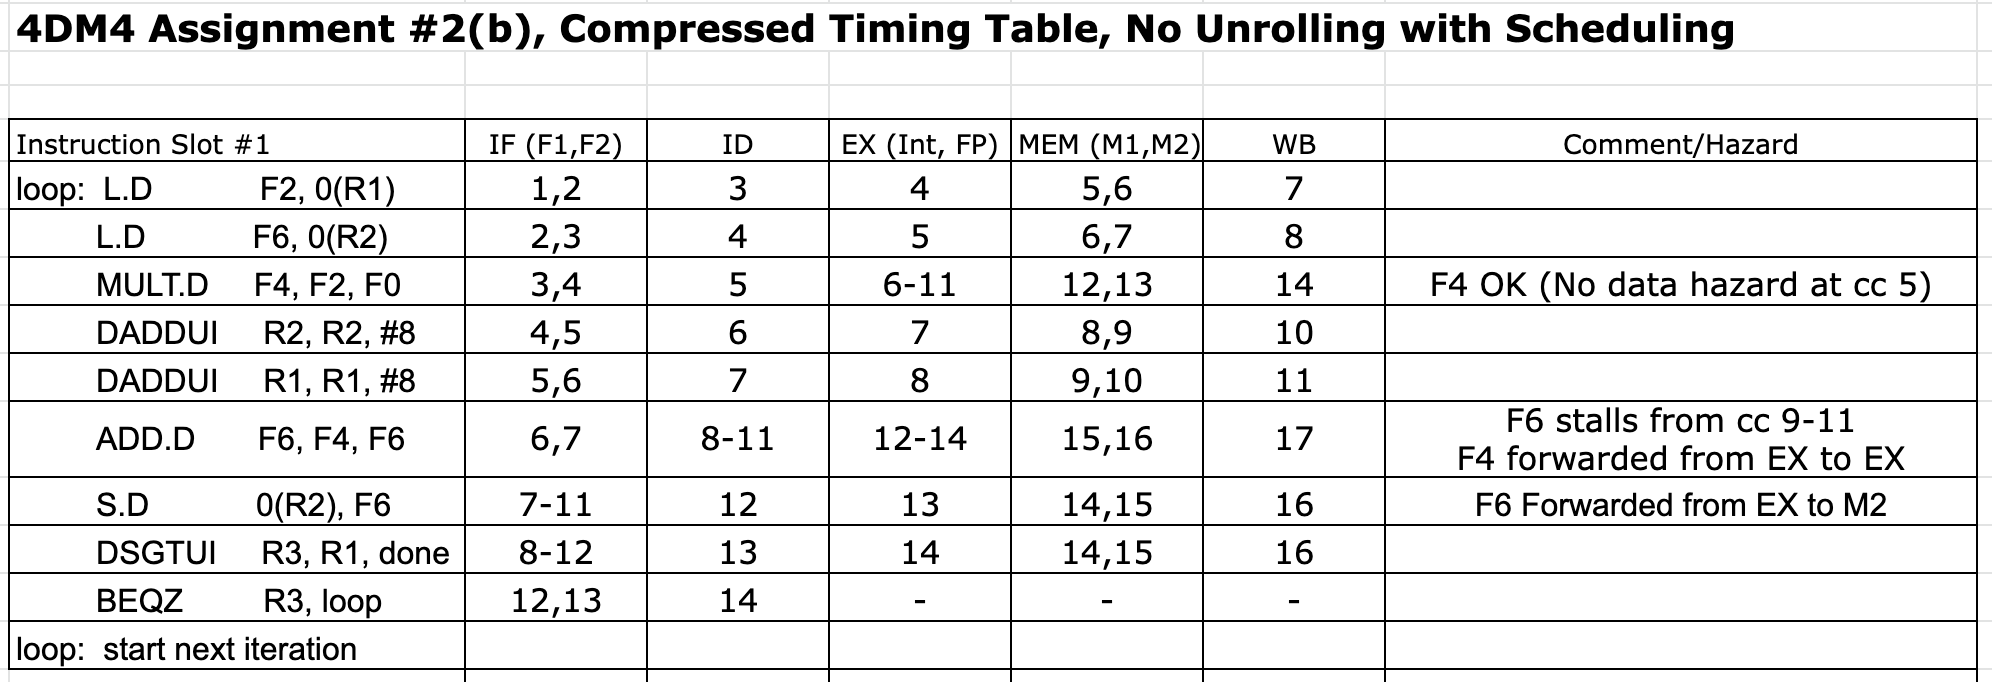
\includegraphics[width=\textwidth]{2b}
	Each iteration of this loop takes 16 clock cycles. The given clock speed is 3 GHz. The following equation can be used to calculate the MFLOP rating for this process.
	\begin{equation}
		\text{MFLOP Rating} = (3 \text{{Ghz}}) * \frac{1 \text{ FLOP}}{16 \text{ clock cycles}} = 187.5 \text{ MFLOP/s}
	\end{equation}

\section{Part (c): DAXPY Loop, with Unrolling, with No Scheduling}
	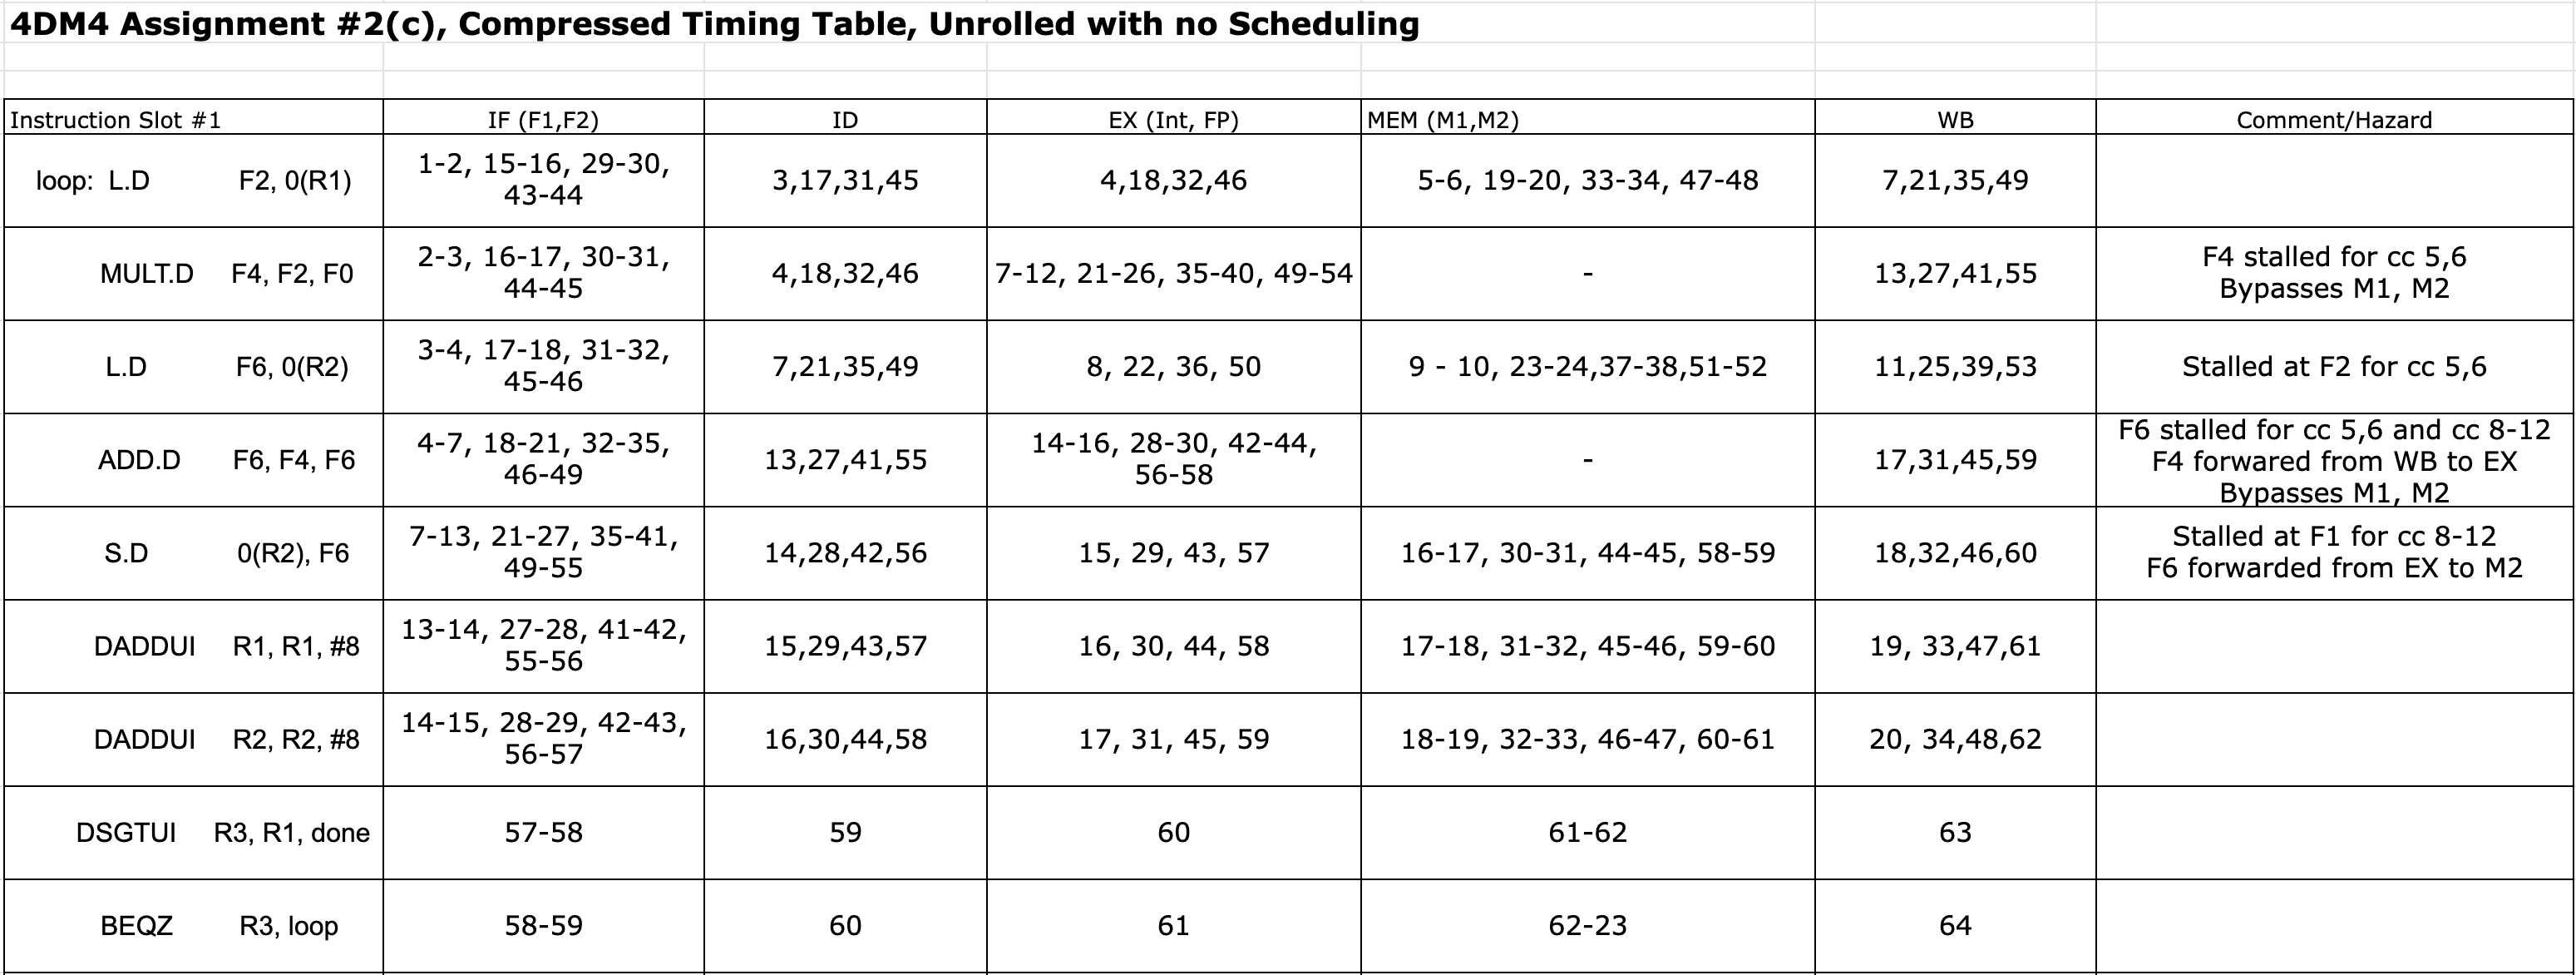
\includegraphics[width=\textwidth]{2c}
	Each iteration of this loop (unrolled 4 times) takes 64 clock cycles. The given clock speed is 3 GHz. The following equation can be used to calculate the MFLOP rating for this process.
	\begin{equation}
		\text{MFLOP Rating} = (3 \text{{Ghz}}) * \frac{1 \text{ FLOP}}{64 \text{ clock cycles}} = 46.9 \text{ MFLOP/s}
	\end{equation}

\section{Part (d): DAXPY Loop, with Unrolling, with Scheduling}
	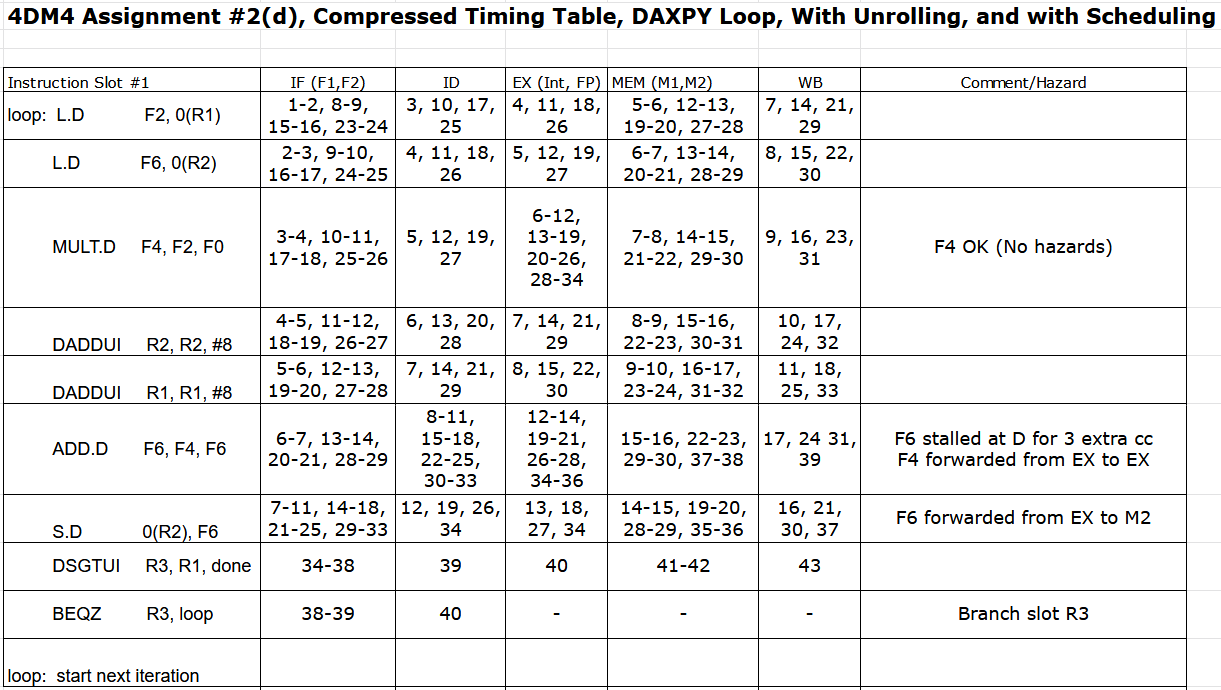
\includegraphics[width=\textwidth]{2d}
	Each iteration of this loop (unrolled 4 times) takes 43 clock cycles. The given clock speed is 3 GHz. The following equation can be used to calculate the MFLOP rating for this process.
	\begin{equation}
		\text{MFLOP Rating} = (3 \text{{Ghz}}) * \frac{1 \text{ FLOP}}{43 \text{ clock cycles}} = 69.7 \text{ MFLOP/s}
	\end{equation}
\section{Part (e): DAXPY Loop, with Unrolling, with Scheduling. On  Dual-Issue Machine}
	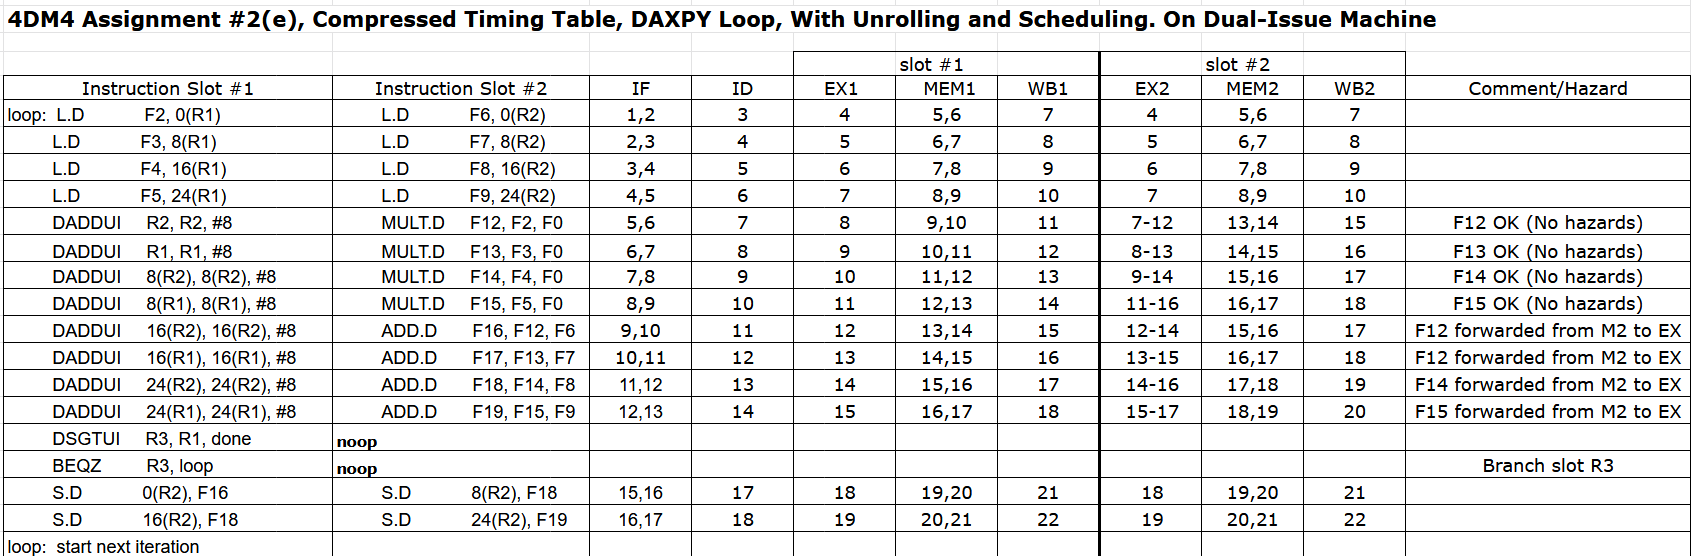
\includegraphics[width=\textwidth]{2e}
	Each iteration of this loop (unrolled 4 times) is ran using 2 seperate slots, allowing for 2 instructions to run simultaneously. The whole iteration takes 22 clock cycles. The given clock speed is 3 GHz. The following equation can be used to calculate the MFLOP rating for this process.
	\begin{equation}
		\text{MFLOP Rating} = (3 \text{{Ghz}}) * \frac{1 \text{ FLOP}}{22 \text{ clock cycles}} = ?? \text{ MFLOP/s}
	\end{equation}



\end{document}